% Chapter Template

\chapter{Ensayos y resultados} % Main chapter title

\label{Chapter4} % Change X to a consecutive number; for referencing this chapter elsewhere, use \ref{ChapterX}
En este capítulo se detallan los ensayos realizados para verificar el correcto funcionamiento del prototipo y el cumplimiento de los requisitos tanto en la etapa digital como en la analogica.
%----------------------------------------------------------------------------------------
%	SECTION 1
%----------------------------------------------------------------------------------------

\section{Banco de pruebas}
Para los ensayos efectuados en laboratorio se montó un banco de pruebas, figura \ref{fig:bancoDePruebas}, constituido por los siguientes elementos:

\begin{itemize}
\item Generador DDS FY6900,
\item Cable BNC-SMA (Canal descarga parcial)
\item Cable BNC-Cocodrilos (Canal senoide de referencia)
\item Computadora portátil. 
\item Puerto serie-USB
\item Prototipo funcional.
\end{itemize}

\vspace{10mm}

\begin{figure}[ht]
	\centering
	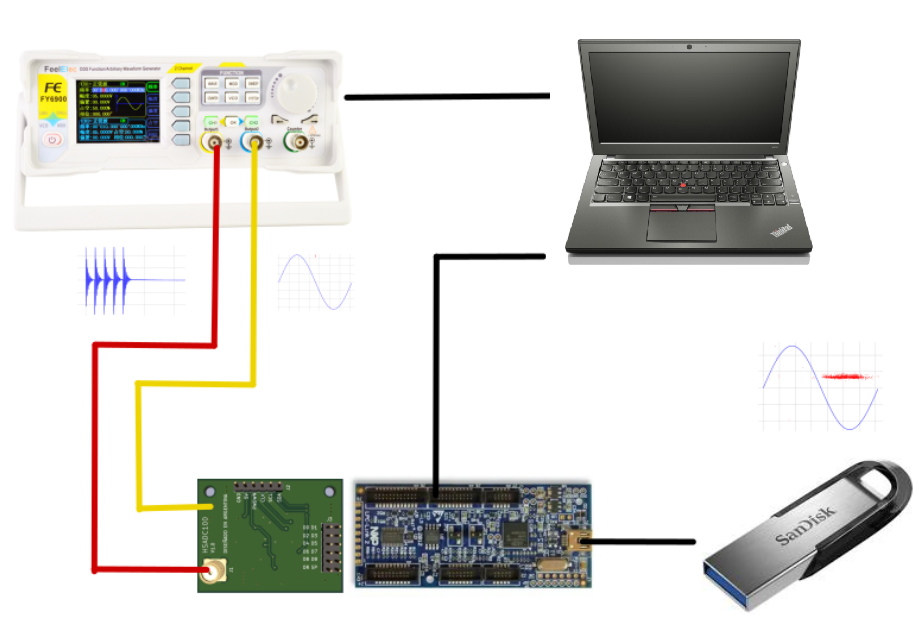
\includegraphics[width=100mm]{./Figures/bancoDePruebas.png}
	\caption{Arquitectura del banco de prueba.}
	\label{fig:bancoDePruebas}
\end{figure}

El banco permitió simular, por medio del generador, la forma de onda de una descarga parcial y sincronizarla con una senoide de referencia de 50Hz. La computadora portátil fue utilizada para acceder por medio del puerto serial a la interfaz de usuario. También se utilizó para controlar al DDS utilizando la base de datos de patrones proporcionada por el cliente. El conjunto de elementos elegidos permitió realizar diversas pruebas manuales y automatizadas.

Debido a las limitaciones del DDS FY6900 los ensayos de validación de amplitud y fase debieron hacerse por separado. Esto fue a causa de que el instrumento no permite realizar demoras en el disparo de un canal con respecto del otro.


\section{Ensayos de amplitud}
Durante los ensayos de amplitud se buscó validar que las señales obtenidas por el prototipo correspondan en amplitud y forma con la señales inyectadas. Para esto se generaron por medio del DDS señales senoidales en diferentes frecuencias y amplitudes.

En las figuras \ref{fig:sin1} y \ref{fig:sin39} se puede observar el efecto de atenuación del filtro comparando la amplitud de entrada y la amplitud medida. Las frecuencias elegidas tienen como objetivo reducir el efecto del sub muestreo cercano a la frecuencia de Nyquist que conlleva a no detectar correctamente los máximos.

\vspace{5mm}

\begin{figure}[ht]
	\centering
	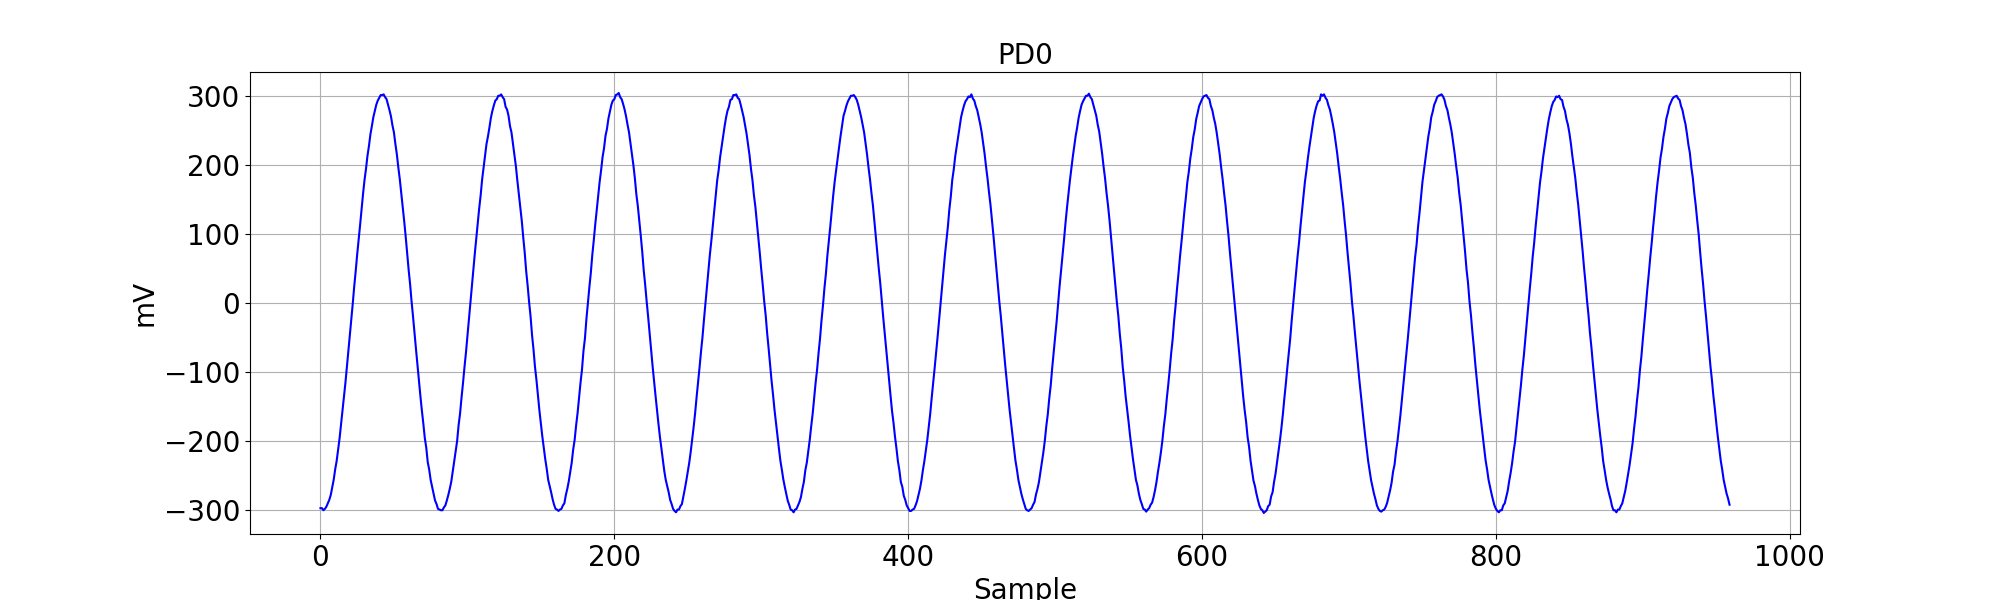
\includegraphics[width=140mm]{./Figures/sin1.png}
	\caption{Seno 1M 600 mVpp.}
	\label{fig:sin1}
\end{figure}

\begin{figure}[ht]
	\centering
	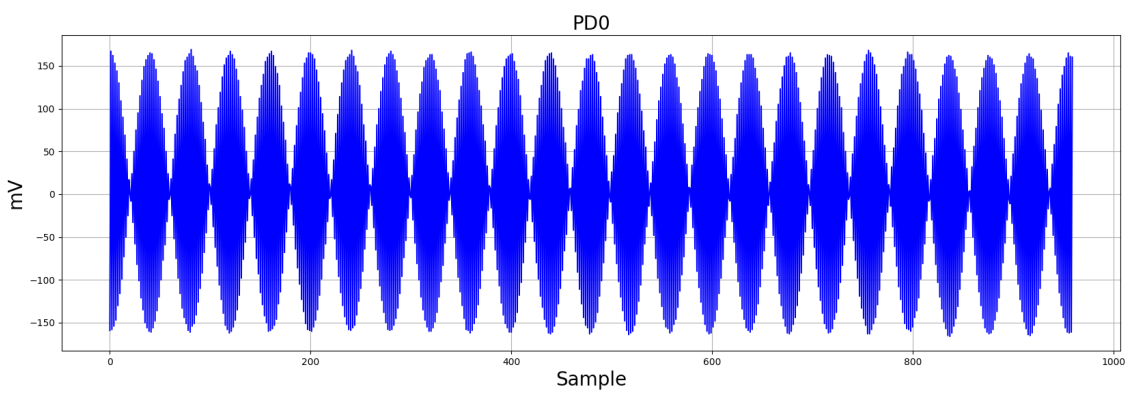
\includegraphics[width=140mm]{./Figures/sin39.png}
	\caption{Seno 39M 600 mVpp.}
	\label{fig:sin39}
\end{figure}

\vspace{5mm}

En la tabla \ref{tab:tensiones} se presentan la máxima tensión de entrada y la máxima tensión de salida para cada frecuencia registrada. Por medio de estos valores se calculó la respuesta en frecuencia del filtro real. 

\begin{table}[h]
\centering
\caption[Antenuación del filtro]{Atenuación del filtro}
\begin{tabular*}{\textwidth}{l c c c c}
\toprule
\textbf{F (MHz)} & \textbf{Entrada (mV)} & \textbf{Salida (mV)} & \textbf{Atenuación (dB)} & \textbf{At. esperada (dB)}\\
\midrule
1 & 600 & 610 & 0,07178584627 & -0,1770 \\
13 & 600 & 580 & -0,147232568 & -0,1770 \\
19 & 600 & 540 & -0,457574905 & -0,1950 \\
25 & 600 & 540 & -0,457574905 & -0,3670 \\
27 & 600 & 540 & -0,457574905 & -0,3670 \\
33 & 600 & 520 & -0,621479067 & -0,5570 \\
39 & 600 & 330 & -2,59637310 & -2,2650 \\
\bottomrule
\hline
\end{tabular*}
\label{tab:tensiones}
\end{table}

\vspace{5mm}

En la figura \ref{fig:respFrecReal} se puede observar la comparativa entre la respuesta del filtro esperada y la deseada

\begin{figure}[ht]
	\centering
	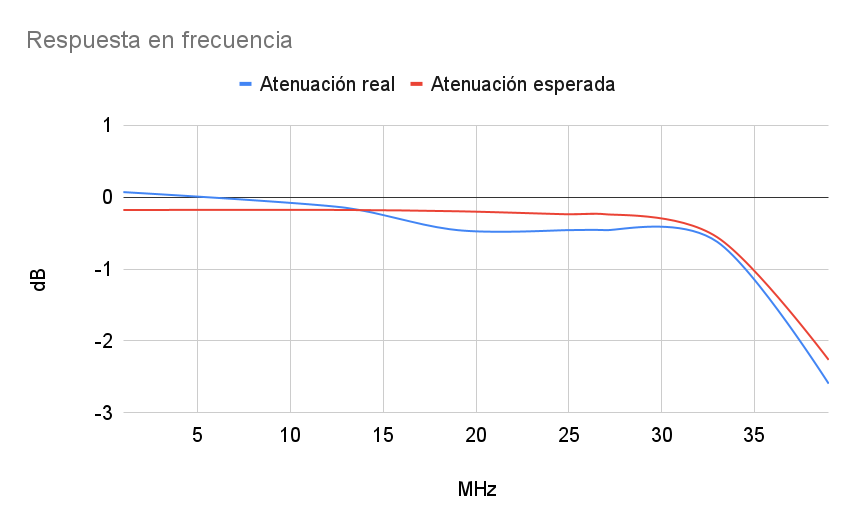
\includegraphics[width=130mm]{./Figures/respFrecReal.png}
	\caption{Respuesta en frecuencia del filtro implementado.}
	\label{fig:respFrecReal}
\end{figure}

\vspace{5mm}


Otra prueba realizada fue la inyección de una descarga parcial sintetizada, figura \ref{fig:dpSint}, utilizando como parámetros una descarga parcial real. 

\begin{figure}[ht]
	\centering
	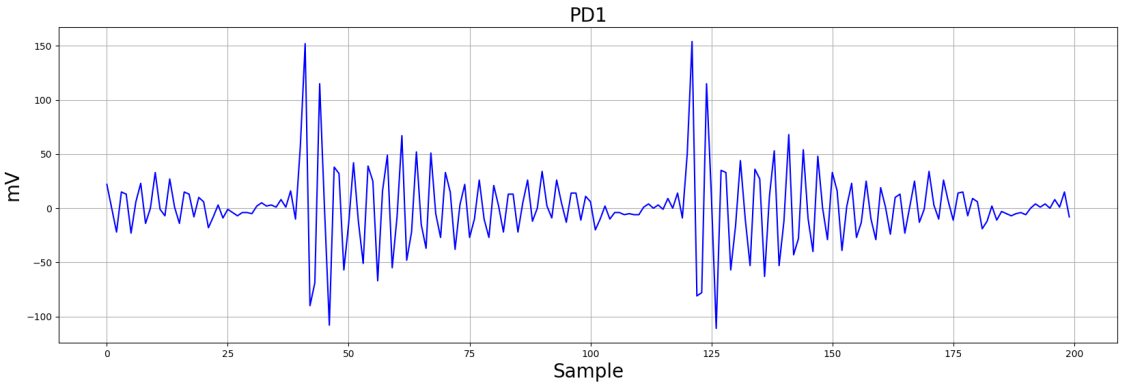
\includegraphics[width=140mm]{./Figures/dpSint.png}
	\caption{DP real sintetizada 400mvpp capturada por el equipo.}
	\label{fig:dpSint}
\end{figure}

La señal original fue muestreada a una tasa de 250 Msps, para poder realizar una correcta comparación de la integridad de la señal se realizó un resampling del pulso adquirido por el equipo a la misma tasa que la original. También se aplicó de forma matemática sobre la señal original la respuesta en frecuencia del filtro de entrada. Ambas señales fueron superpuestas en la figura \ref{fig:compPulsos}.

\begin{figure}[ht]
	\centering
	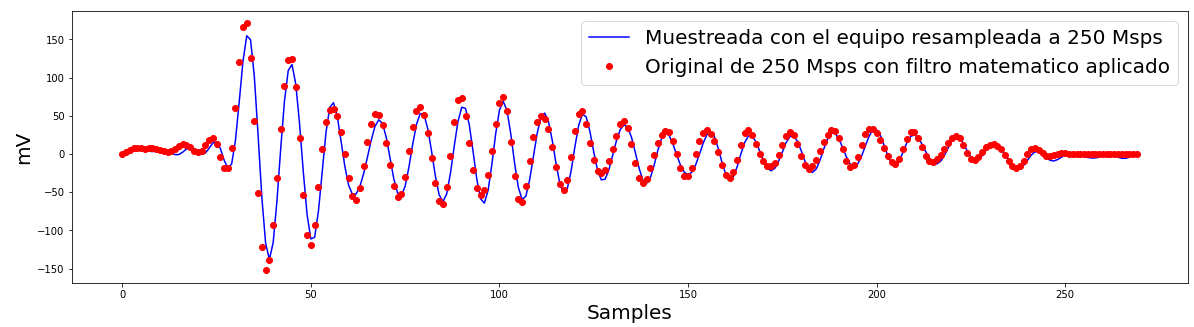
\includegraphics[width=140mm]{./Figures/compPulsos.png}
	\caption{Comparación pulso original y pulso adquirido resampleado.}
	\label{fig:compPulsos}
\end{figure}

\vspace{20mm}

Aplicando la transformada de Fourier sobre las señales de la comparativa anterior se realizó una comparativa de la distribución de energía en el espectro de la frecuencia, figura \ref{fig:compEspectro}.

\vspace{5mm}

\begin{figure}[ht]
	\centering
	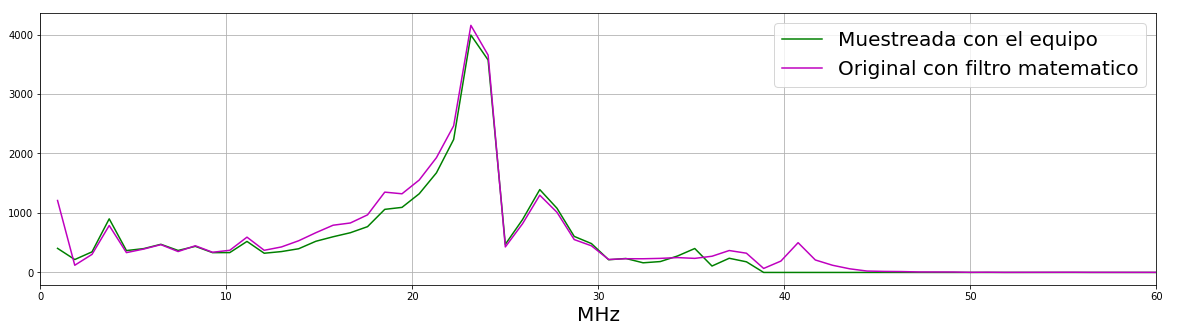
\includegraphics[width=140mm]{./Figures/compEspectro.png}
	\caption{Distribución del espectro.}
	\label{fig:compEspectro}
\end{figure}

\newpage

\section{Ensayos de disparo}
Durante los ensayos de disparo se realizaron mediciones del tiempo requerido por el sistema para poder rearmar su trigger, figura \ref{fig:compEspectro}. Esta latencia se encuentra determinada principalmente por el tiempo requerido para configurar nuevamente los punteros a memoria y reiniciar el periférico ADC de alta velocidad. Durante la adquisición de slots pertenecientes al mismo banco de memoria el tiempo de rearme fue de 90 microsegundos. Considerando que un grado de la senoide de referencia representan 55 microsegundos, la distancia mínima angular adquirible entre descargas parciales será de 1°36’.

\vspace{5mm}

\begin{figure}[ht]
	\centering
	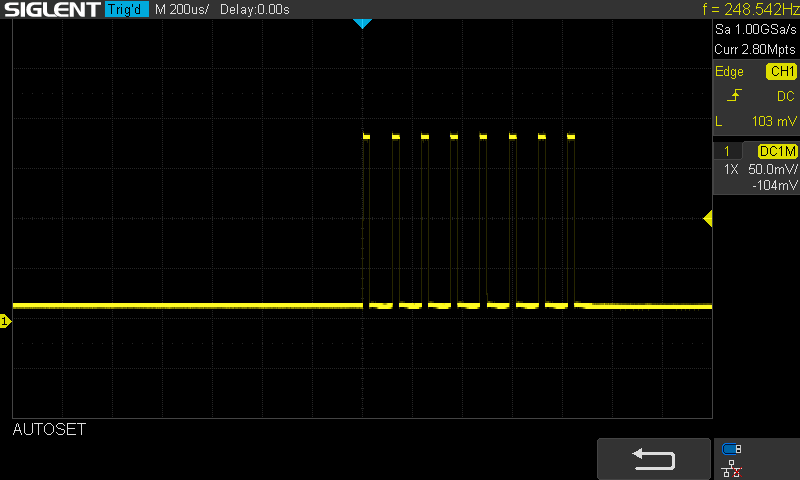
\includegraphics[width=140mm]{./Figures/disparos.png}
	\caption{Adquisición de un banco completo de 8 slots de 2048 muestras.}
	\label{fig:oscDisparos}
\end{figure}

\vspace{5mm}

Además del tiempo requerido para el rearme se realizaron mediciones sobre el tiempo mínimo requerido, por el procesador, para atender el disparo del \textit{trigger}. Este tiempo es de suma importancia porque determinará cuantas muestras de desplazamiento existen desde que el \textit{trigger} detectó su disparo hasta que el procesador pudo atenderlo, figuras \ref{fig:tiempoInicial}. El tiempo mínimo de latencia para un cortex M4 es de 12 ciclos de reloj. Debido a que la velocidad del núcleo es de 204 Mhz y la del el conversor AD es de 80 Mhz se puede determinar que un tiempo mínimo de latencia de 5 muestras. Durante esta etapa también se realizaron pruebas comparativas a fin de determinar el \textit{jitter} entre los diferentes disparos ya que el tiempo de atención de la interrupción depende ademas de como se haya diseñado el firmware y de la utilización de los bancos de memoria ram. El \textit{jitter} medido fue siempre inferior a 4 muestras oscilando normalmente entre 1 y 2 .

\vspace{5mm}

\begin{figure}[ht]
	\centering
	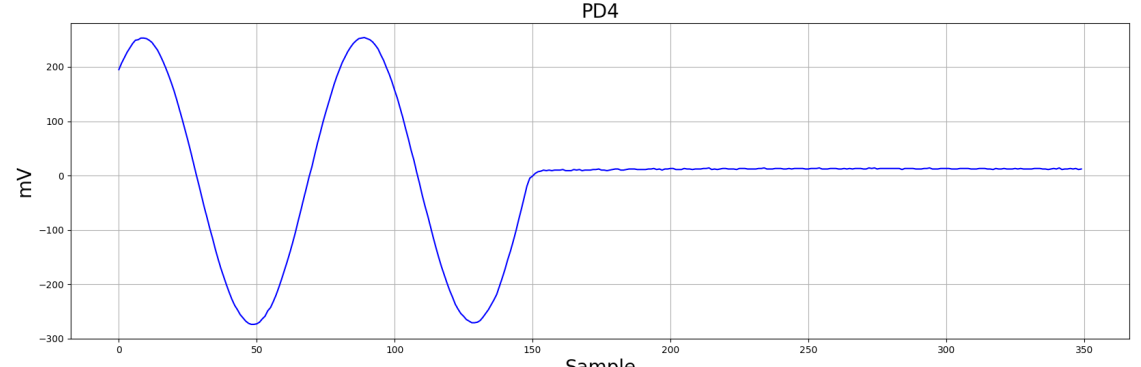
\includegraphics[width=130mm]{./Figures/tiempoInicial.png}
	\caption{Dos ciclos, trigger 200mV y flanco ascendente.}
	\label{fig:tiempoInicial}
\end{figure}


\section{Ensayos de fase}

Los ensayos de fase buscan verificar que la detección de una descarga parcial determinada está vinculada con el momento angular correcto de la senoide de referencia.
Debido a restricciones del banco de pruebas para disparar una senoide sintetizada de alta frecuencia en un momento angular dado de la senoide de referencia, se recurrió a utilizar una señal cuadrada de 50 Hz con un duty cicle del 0,001\% para la señales positivas y de 99,999\% para las negativas. De esta manera la entrada optoacoplada y la entrada de descargas parciales pudieron ser excitadas en forma conjunta durante todo el periodo de la señal de referencia.
Como la señal inyectada en la entrada de descargas parciales no se encuentra dentro de rango lineal del filtro la medición de tensión no se tomará en cuenta para esta prueba.
La figura \ref{fig:rafagaCero} muestra la adquisición de una serie de pulsos de DP disparados en fase 0 de una senoide de referencia de 50 hz.

\vspace{5mm}

\begin{figure}[ht]
	\centering
	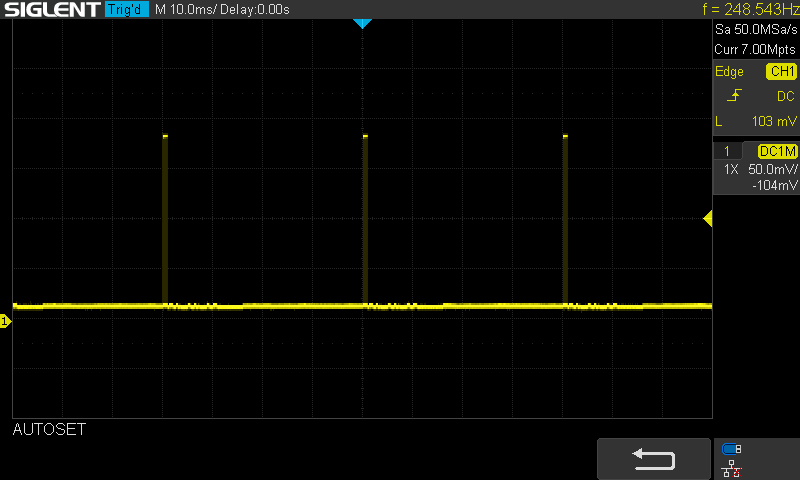
\includegraphics[width=130mm]{./Figures/rafagaCero.png}
	\caption{Rafaga de adquisiciones en el grado 0 de la senoide de referencia.}
	\label{fig:rafagaCero}
\end{figure}

\vspace{5mm}

En la figura \ref{fig:zeroCross} puede verse la comparación entre la senoide de referencia y la salida aislada ópticamente.

\vspace{5mm}

\begin{figure}[ht]
	\centering
	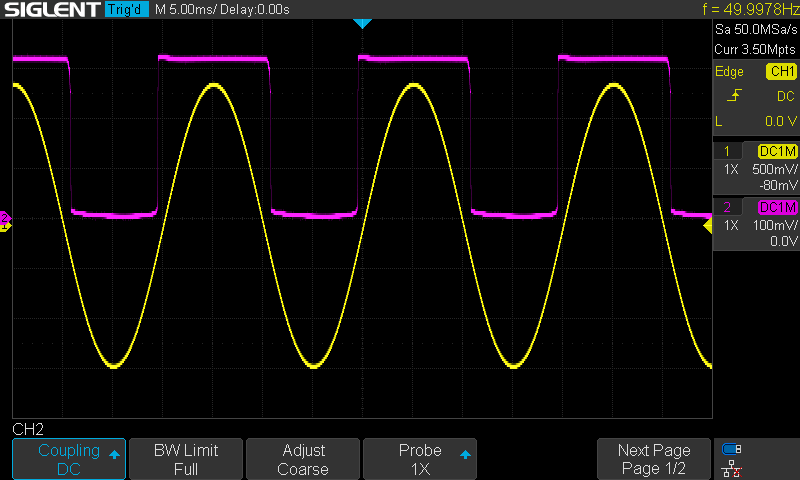
\includegraphics[width=130mm]{./Figures/zeroCross.png}
	\caption{Senoide de referencia y salida de detección de cruce por 0 optoacoplada.}
	\label{fig:zeroCross}
\end{figure}

\vspace{5mm}

Además de verificar disparos individuales configurados manualmente, se realizó un script en python con la librería fygen capaz de sintetizar un patrón de descargas parciales. Los datos utilizados provienen de archivos matlab que fueron previamente generados en base a mediciones reales realizadas por el cliente.
[https://github.com/mattwach/fygen]
En la figura XX puede verse la comparativa entre el patrón de DP generado por el cliente y el patrón de DP generado por el equipo en base a la misma secuencia de señales sintetizadas. Como difierencia se encuentra que la escala vertical de el patron original se encuentra expresada en pico coulombs y la generada en milivolts, esto se debe a que la magnitud solo fue tomada como referencia por tratarse de un ensayo de fase.


\begin{figure}[htp] 
    \centering
    \subfloat[Corona original.]{%
        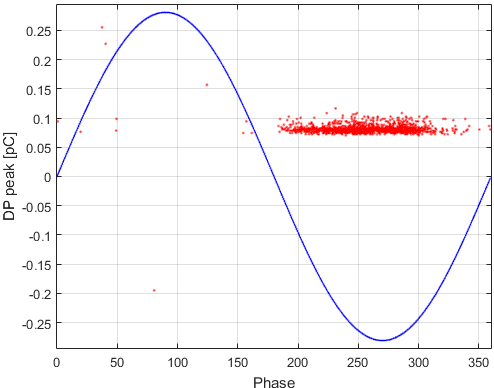
\includegraphics[width=0.46\textwidth]{./Figures/corona1Original.png}%
        \label{fig:corona1Original}%
        }%
    \hfill%
    \subfloat[Corona sintetizada.]{%
        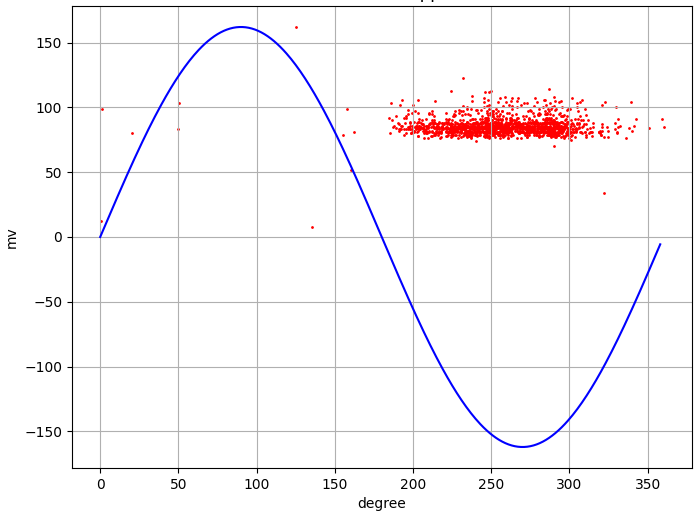
\includegraphics[width=0.5\textwidth]{./Figures/corona1Propia.png}%
        \label{fig:corona1Propia}%
        }%
    \caption{Comparación entre un patrón original y un patrón sintetizado.}
\end{figure}

\begin{figure}[htp] 
    \centering
    \subfloat[Corona original.]{%
        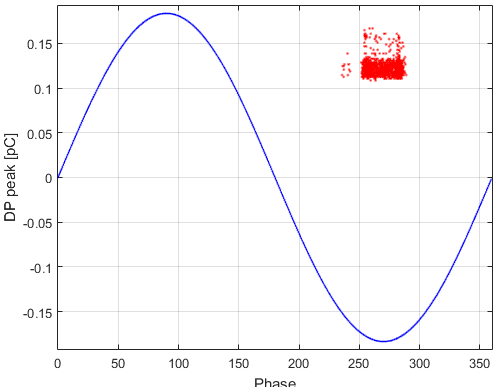
\includegraphics[width=0.475\textwidth]{./Figures/corona2Original.png}%
        \label{fig:corona2Original}%
        }%
    \hfill%
    \subfloat[Corona sintetizada.]{%
        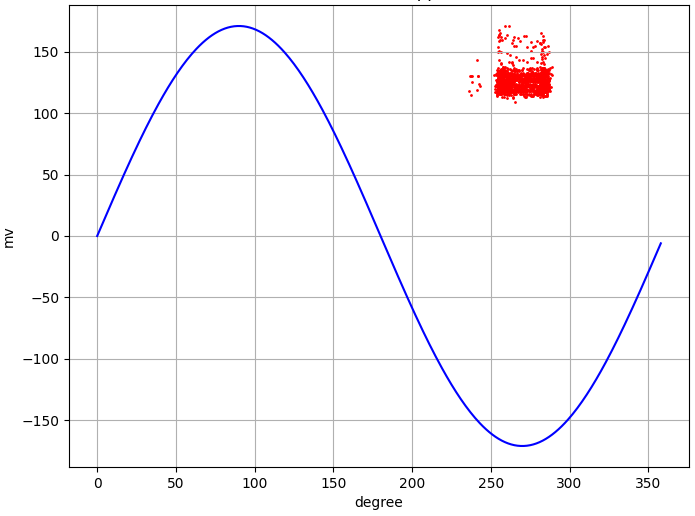
\includegraphics[width=0.5\textwidth]{./Figures/corona2Propia.png}%
        \label{fig:corona2Propia}%
        }%
    \caption{Comparación entre un patrón original y un patrón sintetizado.}
\end{figure}


\section{Tiempos de procesamiento y almacenado}
Los ensayos de tiempo de procesamiento se realizaron utilizando un osciloscopio y un pin de salida como marcador del estado interno del procesador.
Durante este ensayo se buscó cuantificar el tiempo requerido por el procesador para realizar los distintos procesamientos. 
La operatoria de procesamiento se ejecuta al finalizar la adquisición de un bloque de memoria. Durante la misma se recorren los slots en búsqueda del valor máximo absoluto, una vez encontrado se calcula la fase de la senoide de referencia del mismo y se guarda en memoria ram. Para ejecutar este proceso sobre un banco de 16384 muestras, figura \ref{fig:tiempoSavePatron}, es necesario un tiempo de 5,5 milisegundos. Esto equivale a 99 grados de desplazamiento angular de la senoide de referencia. Si el proceso es finalizado antes de comenzar un nuevo semiciclo el procesador puede rearmarse y continuar, de lo contrario deberá dejar un ciclo muerto.

\begin{figure}[ht]
	\centering
	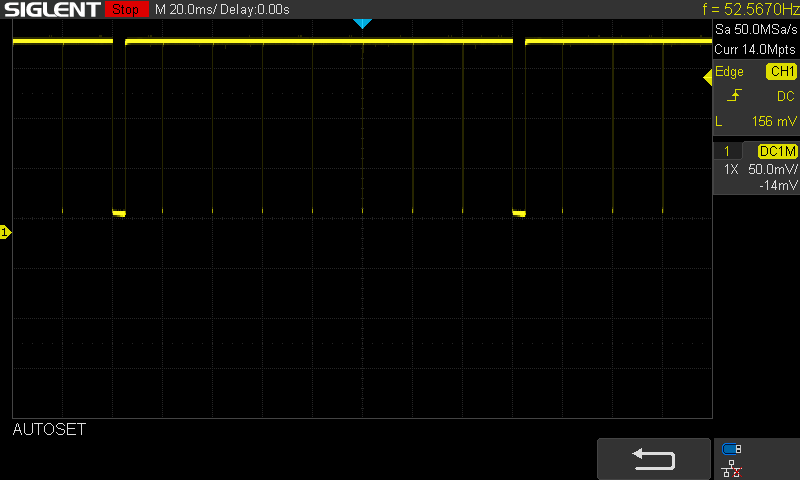
\includegraphics[width=130mm]{./Figures/tiempoSavePatron.png}
	\caption{Tiempo necesario para procesar 8 slots de memoria de 2048 muestras y obtener sus valores máximos absolutos con sus respectivas fases.}
	\label{fig:tiempoSavePatron}
\end{figure}

Los ensayos de almacenamiento se realizaron con el fin de determinar cuánto tiempo requiere el procesador para almacenar el total de la adquisición en el soporte flash USB. Al igual que el procesamiento este proceso se realiza al completar un banco de memoria, por lo que se efectúan rafagas de escritura de 32768 kbytes. Junto con el vuelco de memoria se efectúa el proceso de búsqueda de pico y fase descripto en el ensayo de procesamiento. En la figura \ref{fig:tiempoSaveAll}  se observa que el tiempo requerido para realizar un vuelco de memoria y su procesamiento es de 16 milisegundos, esto es igual a 288° de desplazamiento angular sobre la senoide de referencia. Al igual que en el proceso de procesamiento el sistema podrá rearmarse si finaliza antes del inicio de un nuevo periodo, de lo contrario deberá dejar un ciclo muerto.

\begin{figure}[ht]
	\centering
	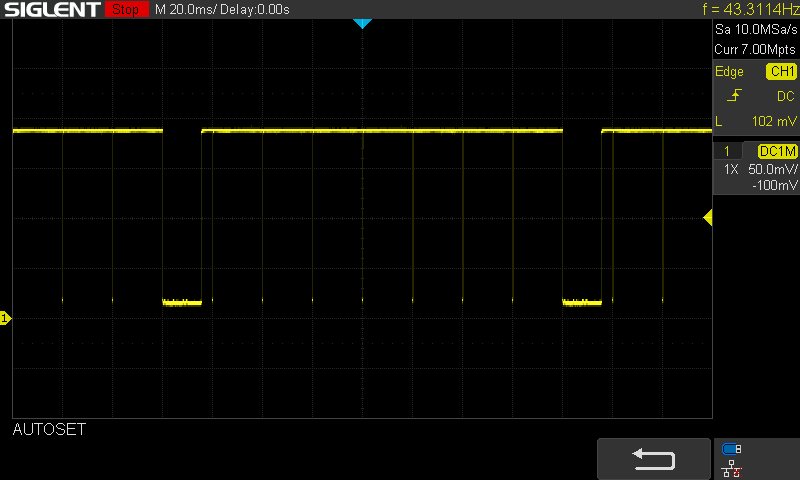
\includegraphics[width=130mm]{./Figures/tiempoSaveAll.png}
	\caption{Tiempo necesario para procesar 8 slots de memoria de 2048 muestras, obtener sus valores máximos absolutos con sus respectivas fases y almacenarlo en la unidad flash USB.}
	\label{fig:tiempoSaveAll}
\end{figure}

\section{Pruebas en campo}
Debido a la pandemia global COVID-19 no fue posible realizar pruebas en campo ni en el laboratorio situado en la Universidad Tecnológica Nacional Regional General Pacheco.